%\documentclass[a4paper]{article}
\documentclass{IEEEtran}

%\usepackage{times}
\usepackage{graphicx}
\usepackage{amsmath,amssymb}

% Any macro definitions you would like to include
% These are not defined in the style file, because they don't begin
% with \bmva, so they might conflict with the user's own macros.
% The \bmvaOneDot macro adds a full stop unless there is one in the
% text already.
\def\eg{\emph{e.g.,}}
\def\ie{\emph{i.e.,}}
\def\etal{\emph{et al.}}
\def\vs{\emph{vs.}}

% macros for referencing figures, tables, equations and sections
\newcommand{\fref}[1]{Figure~\ref{#1}}
\newcommand{\eref}[1]{(\ref{#1})}
\newcommand{\tref}[1]{Table~\ref{#1}}
\newcommand{\sref}[1]{Section~\ref{#1}}
\newcommand{\aref}[1]{Algorithm~\ref{#1}}
\newcommand{\emptybox}[2]{\framebox[#1][l]{\rule[#2]{0pt}{0pt}}}

% maths macros
\def\G{G}
\def\Gx{G_x}
\def\Gy{G_y}
\def\Gxx{G_{xx}}
\def\Gxy{G_{xy}} \def\Gyx{G_{yx}}
\def\Gyy{G_{yy}}
\def\Ix{I_x}
\def\Iy{I_y}
\def\Ixsqr{I_{x^2}}
\def\Iysqr{I_{y^2}}
\def\Ixx{I_{xx}}
\def\Ixy{I_{xy}}
\def\Iyy{I_{yy}}
\def\dtcwt{DT-$\mathbb{C}$WT}

\def\deg{\ensuremath{^\circ}}
\def\rad{\ensuremath{\text{radians}}}
\def\by{\ensuremath{\times}}

% lengths for image sizes
\newlength{\qtrcol}\setlength{\qtrcol}{0.24\columnwidth}
\newlength{\halfcol}\setlength{\halfcol}{0.48\columnwidth}

% command for adding inline comment to text
\newcommand{\comment}[1]{}

% define title here so headers are updated, too
\def\ttl{Analysing Curvilinear Structures in Images}
\title{\ttl}
\author{Authors}

% define path to figures
\def\figroot{./figs}
\def\figpath{\figroot}


%-------------------------------------------------------------------------
% Document starts here
\begin{document}

\tableofcontents\clearpage

\maketitle

\begin{abstract}
Estimating orientation of image structure underpins applications including digital mammography, retinography and fingerprint analysis. We consider different choices of filter bank including those based on first and second derivatives, efficient Haar-like features and the Dual Tree Complex Wavelet Transform. We then investigate how standard regressors (linear regression, Boosting and Random Forests) may be adapted to use the responses to these filter banks in order to predict orientation of image structure. For a quantitative evaluation, we use synthetic images based on mammograms and the publicly available DRIVE database of retinal images, and show that Random Forests and the wavelet transform offer superior accuracy though at a cost in efficiency. Qualitative results are also presented for real mammograms and fingerprint images.
\end{abstract}

% Put in any papers to be referenced in here.
% This will give us an idea of how many we have in total and how much space the references take up

\nocite{Kovesi_DICTA03}
\nocite{Amin_Yan_ICMLC09}
\nocite{Wang_etal_PRL11}



\section{Introduction}
% State the problem, and its impact on all stakeholders (those directly affected, and society at large e.g. the social and economic impact of treating the disease)
A curvilinear structure in an image appears as a ribbon or bar of finite width that is distinguishable from the surrounding structure, with a cross-sectional profile that is repeated along a linear, though not necessarily straight, path (\fref{f:line_examples}).

%What are their general characteristics?
%Defined locally by their cross-sectional profile and orientation, and assumed to extend in at least one direction normal to the profile (as opposed to a blob).

Detecting and measuring the properties of curvilinear structures in images is useful for many reasons~\cite{Ayres_Rangayyan_JEI07}:

\begin{itemize}
\item detecting distinctive patterns of vessels and fibrous tissue can improve quality of life and reduce costs associated with treating diseases such as retinopathy (\sref{s:retinopathy}) and breast cancer (\sref{s:mammography}) in advanced stages by aiding early diagnosis and treatment; %
\item spotting cracks and other similar defects in manufactured items such as roads, eggs can reduce costs associated with waste; %
\item biometrics based on ridge patterns in fingerprints~\cite{}, or the veins of the finger~\cite{} or hand~\cite{}, can bring criminals to justice and prevent further crime, or enhance the usability of technology by controlling access to sensitive data; %
\item detecting roads, railways and rivers in aerial photography can help to build maps automatically for applications such as providing relief in remote areas following a natural disaster.
\end{itemize}


\subsection{Aims and Objectives}
% Specific aims of the study
Given an image, our aim is to determine where any linear structures exist in the image, and to measure values that correspond to low-level properties such as orientation, width, and cross-sectional profile. Although these properties form the basis of higher level, application-specific analysis (classifying structure as \emph{road}, \emph{rail} or \emph{river} in aerial photographs, for example), our focus is purely on computing the local attributes as accurately and robustly as possible; by improving the accuracy of the values we estimate, it follows logically that performance should improve for all higher level analysis methods that use these values as inputs.\footnote{Any algorithm that does not benefit from better input should be regarded with suspicion.}

%For example, any method to move from a map of vessel probabilities and predicted orientations in a retinograms, to an explicit grouping of pixels that belong to individual vessels, is likely to benefit from a priori knowledge of the spatial arrangement vessels in that image class and the physical model of how vessels grow and bifurcate. Such a method will therefore be very different from that needed to group a similar set of local information into the road, rivers etc present in an image for aerial analysis

With this focus, we have two objectives: extract, at every image location, structural information that is rich enough to capture the underlying image properties yet sparse enough to be computed efficiently; and combine this raw local information to predict output values of interest (such as orientation).


% Review other people's attempts at solving the problem, and why they are found wanting
\subsection{Related Work}
\comment{
There is no 3D analogue of the \dtcwt{}. Therefore, we should avoid 3D datasets and related work as much as possible - this paper is solely about the analysis of 2D image structures. This includes aerial photography, retinal images, fingerprints and palmprints, surface inspection, and possibly fibre analysis.
}

Because previous attempts at detecting and measuring curvilinear structures have been surveyed elsewhere, from the general~\cite{Papari_Petkov_IVC11} to the application-specific~\cite{Kirbas_Quek_ACMCS04,Lesage_etal_MIA09}, here we briefly review only a few papers in applications areas of specific interest. We will also discount the very basic detection methods that simply threshold an image~\cite{Jiang_Mojon_TPAMI03} and very complex methods that use techniques such as phase fields~\cite{Peng_etal_IJCV09}, leaving us free to focus on the most popular approaches that apply a bank of filters to the image before interpreting the responses in a way that accentuates the `lineness' at every pixel.

Early examples modelled a curvilinear structure as an image `ridge', typically defined using second order derivatives and formulated either as a Hessian problem~\cite{Frangi_etal_MICCAI98,Sato_etal_MIA98} or as responses to a derivative filter~\cite{Staal_etal_TMI04,Aylward_Bullitt_TMI02,Steger_TPAMI98,Koenderink_vanDoorn_TPAMI92}. Interpreting the responses to these filters used hand-crafted equations based on the differential geometry of the image `surface'~\cite{Frangi_etal_MICCAI98,Sato_etal_MIA98}.

With the maturing of machine learning, it was recognized that hand-crafting could be replaced by flexible statistical models whose parameters were optimized to agree with input-output training example pairs; Gaussian mixture models~\cite{Soares_etal_TMI06}, %
artificial neural networks~\cite{Marin_etal_TMI11,Minh_Hinton_ECCV10}, %
support vector machines~\cite{Ricci_Perfetti_TMI07,Gonzalez_etal_CVPR09}, and %
$k$-nearest neighbour classifiers~\cite{Staal_etal_TMI04} were all popular choices. Not only are these methods well-established and understood within machine learning, but a learnt statistical model can also accommodate different sensing modalities (with different noise properties) and other `stuff' that is hard to hand-craft, making the resulting algorithms more easily transferrable.

In addition, learnt statistical models can be applied to \emph{any} vector of image features to predict the quantity of interest, and are not tied to a particular feature type with specific theoretical properties. Furthermore, flexible statistical models permit the option to include hand-crafted, application-specific features where beneficial~\cite{Staal_etal_TMI04}. As a result, subsequent studies were free to use alternative filter banks and features based on %
matched filters or templates~\cite{Chaudhuri_etal_TMI89,Pechaud_etal_CVPR09,Dixon_Taylor_IPC79,Hoover_etal_TMI00,Ricci_Perfetti_TMI07}; %
derivatives of a first~\cite{Cai_Chung_MICCAI06} or higher than second~\cite{Gonzalez_etal_CVPR09} order; %
Gabor filters~\cite{Soares_etal_TMI06,Dabbah_etal_MIA11}; %
moments~\cite{Marin_etal_TMI11}; %
principal component analysis~\cite{Minh_Hinton_ECCV10}; %
wavelet transforms; %
and the monogenic signal. %
Some of these filter banks have been evaluated previously in a brief comparison~\cite{Ayres_Rangayyan_JEI07}, though the authors admit that not all filters were compared exactly on a like-for-like basis; our work builds on this comparison.

As well as permitting flexibility in the choice of input feature vector, learnt statistical predictors can be used to predict more than just the presence of a line. In recent studies, for example, orientation~\cite{Zwiggelaar_etal_TMI04,Ayres_Rangayyan_JEI07}, width~\cite{Steger_TPAMI98,Zwiggelaar_etal_TMI04} and multi-class labels~\cite{Zwiggelaar_etal_TMI04} have all been predicted from image feature vectors.

Other facets of tube detection and measurement are interesting though not directly relevant to this work: %
detecting lines at multiple scales~\cite{Lindeberg_IJCV98,Sato_etal_MIA98}; %
dealing with junctions and bifurcations where multiple lines meet at a point~\cite{Chen_etal_TPAMI00};
regularizing estimated lines via snakes~\cite{Laptev_etal_MVA00} or dynamic programming~\cite{Gruen}; %
and line following or tracking~\cite{Aylward_Bullitt_TMI02,Perez_etal_ICCV01}.



% Describe what we do, and why it is better than preceding works
\subsection{Our Contributions}
% Briefly outline our attempt at solving the problem, and why it should be better than the solutions that have preceded it
This paper presents three contributions that advance the current body of knowledge in the analysis of curvilinear image structures.

First, we provide a detailed comparison of commonly used image filter banks in the context of their suitability for extracting the local image information pertaining to curvilinear structure. In doing so, we describe the desirable properties of a suitable filter bank, therefore enabling us to make a principled choice that balances the richness of the extracted information against efficiency (both computational and storage). This analysis leads us to apply a previously unexploited image filter -- the dual-tree complex wavelet transform (\dtcwt{}) -- to the task of curvilinear feature analysis. The \dtcwt{} benefits from specific properties, such as efficiency and phase information, that address the shortcomings of existing popular image filters (\sref{s:filtering}).

Second, we investigate and compare supervised learning approaches that, after training on a set of (input feature vector, target label) example pairs, turn a previously unseen feature vector of filter responses at a given location into an estimated output value. Specifically, we include the Random Forest statistical method -- not investigated in any similar study of which we are aware -- to predict outputs, and compare this to techniques that have been previously used. For line detection (\ie~image segmentation), we show that a carefully selected filter bank, coupled with a modern learning method that is capable of dealing with non-linear data, produces results that match or exceed the state-of-the-art without relying on application-specific assumptions to boost performance. For orientation, we show how to formulate the learning problem such that angle wraparound is dealt with correctly, and in doing so produce\comment{ significantly} better estimates than existing methods that compute orientation analytically. In addition, we show how predicting output responses via machine learning allows us to estimate the error associated with the predictions, which we propose may in itself be of use in further processing.

Third, we explore the similarities and differences between these different approaches, and present empirical evidence of which work best in practice for applications including retinography~(\sref{s:retinography}), mammography~(\sref{s:mammography}) and [another?].

In all cases, we back up theoretical claims for filter performance with thorough experimental validation on both synthetic and real data. 

%Finally, if for a given image class we know of additional properties that will be useful to predict and that can be reliably labelled on our training data (for example, a further classification of structure in aerial images to roads and rivers) these can easily be added to our protocol. 





\clearpage
\section{Input Image Features}
\label{s:filtering}
To predict some quantity of interest (such as line orientation or the probability of linear structure) from a sample image patch, it is useful first to reduce the high-dimensional image data to a more compact feature vector that captures the most important properties of the image yet discards redundant information. This improves the performance of statistical pattern recognition algorithms by reducing the effects of the `curse of dimensionality'~\cite{Bellman} whereby the number of training examples required for a given sampling density increases exponentially with input dimensionality.

%Other approaches to detecting linear structure in mammograms include using second derivatives of the mammographic image surface~\cite{Cerneaz_Brady_CVVRRM95} or second derivatives of the 2D Gaussian~\cite{Karssemeijer_teBrake_TMI96}

% Summary: template matching is pretty pants - you only get a strong response if you have the template at the correct location, orientation and scale; steerable filters give you a strong response at the correct location and scale, but orientation can be interpolated from a small number of filters; gabor filters give a strong response at the correct orientation and scale, but can interpolate over small displacements, making them less sensitive to location; the dtcwt can be seen as an efficient approximation to Gabor filters in that must be applied at the correct scale and orientation but uses phase to make it insensitive to displacements. (Can the DTCWT interpolate over orientation, too?)

\subsection{Template Matching}
Template matching approaches take a template that resembles the object of interest, and convolve it with the image at several scales and orientations. A discretized translation, scale and orientation can then be found from local maxima of the filter responses in the four-dimensional parameter space.

\label{s:filtering_linop}
The \emph{line operator}, or `LinOp'~\cite{Dixon_Taylor_IPC79}, is a variant of template matching that uses the responses to a template applied at multiple orientations and scales to describe an image patch. 

\begin{figure}[t]
\centering
\includegraphics[width=0.2\columnwidth]{\figpath/filtering/linop}
%
\caption{LinOp template.}
\label{f:filters_linop}
\end{figure}

% Mammography examples
Though originally applied to detecting asbestos fibres, it was later shown that LinOp could be na\"ively applied to mammograms~\cite{Parr_etal_SPIE97}, and also achieved the highest area under the receiver operating characteristic (ROC) curve in a comparison of methods using simulated mammograms~\cite{Zwiggelaar_etal_TMI04}.
%

Though straightforward to implement, template matching is computationally inefficient due to the need to apply the template at many discrete orientations. Though the number of orientations can be reduced, this reduces the accuracy of the orientation estimate.

\subsection{Steerable Filters}
Applying many filters at discrete orientations can be avoided by using \emph{steerable} filters~\cite{Freeman_Adelson_TPAMI91,Koenderink_vanDoorn_TPAMI92}, where the response to a filter at any angle can be computed as a function of the response to the filter at a small and fixed number of orientations. Not only does this provide almost arbitrary accuracy for a fixed number of oriented basis filters, but the basis filters are frequently \emph{separable}, making the convolution itself more efficient. Here we consider two popular choices: first- and second-order derivatives of the Gaussian.

\subsubsection{First order derivatives}
\label{s:filtering_firstderivs}
%
\input{methods/image_processing/fig_filtering_firstderivs}%
%
Horizontal and vertical first-order derivatives of a Gaussian kernel, $\Gx$ and $\Gy$ (\fref{f:filters}a), give a smoothed estimate of the image gradient in $x$ and $y$, and are used in many edge detectors (\eg~Canny~\cite{Canny_TPAMI86}). These filters are separable, such that the filter convolution is highly efficient, and they also form a basis pair for a steerable filter such that the response to the filter at an arbitrary angle, $\theta$, is given by
%
\begin{equation}
R(\theta) = \Ix \cos(\theta) + \Iy \sin(\theta)
\label{e:firstderivs_response}
\end{equation}
%
\noindent where $\Ix=\Gx\ast I$ and $\Iy=\Gy\ast I$ are the image responses to $\Gx$ and $\Gy$, respectively. This response function has two stationary points in the range $[0,2\pi)$, occuring at
%
\begin{equation}
\theta = \tan^{-1}(\Iy/\Ix),
\label{e:firstderivs_orientation}
\end{equation}
%
\noindent that correspond to the equal and opposite directions of maximum absolute gradient.

Though these filters are effective for estimating orientation at an edge, there is an instability when both $\Ix$ and $\Iy$ are close or equal to zero. Unfortunately, this occurs at the centre of a symmetric image feature, such as a bar or ridge, whose orientation we may wish to estimate.
%

%\subsubsection{Squared responses}
%This problem can be avoided by considering the squared response to $G_{(1)}(\theta)$:

\begin{align}
R_{(1)}^2(\theta)
	&=	(\Ix \cos(\theta) + \Iy \sin(\theta))^2 \\
	&= 	\Ix^2 \cos^2(\theta)+\Iy^2 \sin^2(\theta)+2\Ix\Iy\sin(\theta)\cos(\theta) \\
	&= 	\Ix^2 \cos^2(\theta)+\Iy^2 \sin^2(\theta)+\Ix\Iy\sin(2\theta)
\label{e:R1sqr}
\end{align}

\noindent such that differentiating and equating to zero gives
%
\begin{align}
\frac{d}{d\theta}R_{(1)}^2
	&= 	-2\Ix^2 \cos(\theta)\sin(\theta) + 2\Iy^2 \sin(\theta)\cos(\theta) + 2\Ix\Iy\cos(2\theta) \\
	&= 	(\Iy^2-\Ix^2) \sin(2\theta) + 2\Ix\Iy\cos(2\theta) = 0 \\
\Rightarrow \tan(2\theta)
	&= 	\frac{2\Ix\Iy}{\Ix^2-\Iy^2}.
\label{e:t1sqr}
\end{align}

\noindent where, by doubling the angle, opposite orientations reinforce each other rather than cancel out~\cite{Mardia_Jupp_00}. 
%
%
\subsubsection{Second derivatives}
\label{s:filtering_secondderivs}
%
\begin{figure}[t]
\centering
\begin{tabular}{@{}c c c c@{}} % @{} removes padding around the edge of the table
\includegraphics[width=0.2\columnwidth]{\figpath/filtering/Gxx} &
\includegraphics[width=0.2\columnwidth]{\figpath/filtering/Gyy} &
\includegraphics[width=0.2\columnwidth]{\figpath/filtering/Gxy} &
\includegraphics[width=0.2\columnwidth]{\figpath/filtering/Gxx-Gyy} \\
(a) & (b) & (c) & (d)
\end{tabular}
%
\caption{(Second derivatives (a) $\Gxx$ (b) $\Gyy = \Gxx^T$, (c) $\Gxy$, and (d) $\Gxx-\Gyy$.}
\label{f:filters_secondderivs}
\end{figure}%
%
The directional second-order derivative of a Gaussian generates an even (\ie~symmetric) image filter that resembles a bar or ridge feature. Like their first-order counterparts, second-order derivatives are steerable though they require three rather than two basis filters. The second-order basis filters are not separable, though a different formulation generates three equivalent basis filters -- $\Gxx$, $\Gyy$ and $\Gxy$ (\fref{f:filters_secondderivs}) -- that are. The response to a second-order derivative is given by
%
\begin{equation}
R(\theta) = \Ixx \cos^2(\theta) + \Iyy \sin^2(\theta) + \Ixy \sin(2\theta)
\label{e:secondderivs_response}
\end{equation}
%
\noindent where $\Ixx = \Gxx\ast I$, $\Iyy = \Gyy\ast I$ and $\Ixy = \Gxy\ast I$ are the responses to the three separable filters. This response function has four stationary points in the range $[0,2\pi)$, occuring at
%
\begin{equation}
\theta = \frac{1}{2} \tan^{-1}\left( \frac{2\Ixy}{\Ixx-\Iyy} \right).
\label{e:secondderivs_orientation}
\end{equation}
%
\noindent Two of these points, separated by $\pi\,\rad$ because the filter is rotationally symmetric, correspond to the directions in which the filter is aligned with the feature and the \emph{absolute} value of the response is maximal; the other two points correspond to the two perpendicular directions. 

Because, however, the maximal absolute response may correspond to either a maximum or minimum (depending on whether the underlying feature is light-on-dark or vice versa) the only way to find out which of the two perpendicular directions has maximal absolute value is to evaluate the response at both and choose the direction corresponding to the larger absolute value. As a result, estimating orientation from second-order derivatives becomes a nonlinear problem.

Estimating direction or orientation from second-order derivatives also suffers from an instability when both $\Ixy$ and $\Ixx-\Iyy$ are close to zero. Unfortunately, this happens at edges, whose orientation we may wish to estimate.

Efficient approximations to computing second-order derivatives of the Gaussian can be achieved through Haar-like approximations to the derivative filters~\cite{Bay_etal_CVIU08} or by approximating the Gaussian filter and applying local finite differences~\cite{Kovesi_DICTA10}.%

\comment{Haar-like approximations are not as new as I first hoped - they are the basis of the SURF feature descriptor, and Peter Kovesi also wrote a paper explaining why even this is not the most efficient thing to do. I've removed it until we can justify having it in.}
%\subsection{Haar-like Approximations}
%\label{s:filtering_haar}
%
%\begin{figure}[t]
\centering
\begin{tabular}{@{}c c@{}} % @{} removes padding around the edge of the table
\includegraphics[width=0.2\columnwidth]{\figpath/filtering/Gx} &
\includegraphics[width=0.2\columnwidth]{\figpath/filtering/Gy} \\
(a) & (b)
\end{tabular}
%
\caption{First derivatives (a) $\Gx$ and (b) $\Gy = \Gx^T$}
\label{f:filters_firstderivs}
\end{figure}%

When using second derivatives, orientation can be computed analytically from the responses, $\Ixy$ and $\Ixx-\Iyy$, to the filters $\Gxy$ and $\Gxx-\Gyy$, respectively. These filters have a distinctive `cloverleaf' appearance that can be approximated by highly efficient Haar-like features that have demonstrated considerable success in applications such as face detection~\cite{Viola_Jones_IJCV04}. To approximate the latter filter, $\Gxx-\Gyy$, we used a modification of the summed area table to compute features at $45^\circ$~\cite{Lienhart_Maydt_ICIP02}.

One downside to this approach is that when using responses to second derivatives (or their Haar-like approximation) we must compute the responses at the two possible solutions to determine which is the correct one. With the Haar-like approximation that combines the response to $\Ixx$ and $\Iyy$, this analytic solution is no longer available and a regression approach becomes necessary.
% i.e. there is no analytic solution when using a Haar-like approximation%

\subsection{Incorporating Phase}
Because first-order derivatives perform well at edges but poorly at the centre of a line, and second-order derivatives have the opposite characteristics, it is sensible to combine their strengths by using both odd and even filters. Ideally, this would be achieved using a Hilbert Transform pair of filters that are $90\deg$ out of phase, though in practice an approximation is often sufficient~\cite{Freeman_Adelson_TPAMI91}. Information on the \emph{phase} offset of the image feature then becomes available, which can be used to describe the local shape of the linear feature and provide invariance to small displacements from the line centre when estimating orientation.

%Researchers have recognised the importance of using local phase information to distinguish between strong edges and genuine curvilinear structure. In mammography, examples include Gabor filters~\cite{Rangayyan_Ayres_MBEC06} and other sets of complex filters~\cite{Schenk_Brady_IWDM02,McLoughlin_etal_SPIE02} that were also steerable~\cite{Freeman_Adelson_TPAMI91}, at multiple scales to compute local energy, orientation and phase at each pixel. 

%One further study used the `monogenic' signal~\cite{Wai_etal_MICCAI04} as a more efficient way of calculating local phase and orientation at multiple scales, detecting curvilinear structure using amplitude-weighted local phase congruency.

Here we consider three approaches that combine the strengths of odd and even filters: the monogenic signal; Gabor wavelets~\cite{Daugman_TASSP88}; and the Dual Tree Complex Wavelet Transform (\dtcwt{}~\cite{Kingsbury_PTRSLA99}), so far unexploited in applications analysing curvilinear structure.

\subsubsection{The Monogenic Signal}
\label{s:filtering_monogenic}
%
\comment{If we need the space, I'd consider reducing this to a paragraph that states that the monogenic signal suffers the same problems as first derivatives, despite its use of phase.}
%
\begin{figure}[t]
\centering
\begin{tabular}{@{}c c c@{}} % @{} removes padding around the edge of the table
\includegraphics[width=0.2\columnwidth]{\figpath/filtering/mono_b} &
\includegraphics[width=0.2\columnwidth]{\figpath/filtering/mono_hx} &
\includegraphics[width=0.2\columnwidth]{\figpath/filtering/mono_hy} \\
(a) & (b) & (c)
\end{tabular}
%
\caption{Monogenic signal filters (a) $B$, (b) $h_x$, and (c) $h_y = h_x^T$.}
\label{f:filters_monogenic}
\end{figure}
%
The monogenic signal~\cite{Felsberg_Sommer_TSP01} computes phase and orientation at a given image location using three filters: one even band-pass filter $B$, and an odd quadrature pair of filters $h_x(x,y) = x/f(x,y)$ and $h_y(x,y) = y/f(x,y)$ where $f(x,y) = 2\pi(x^2 + y^2)^{\frac{3}{2}}$ (\fref{f:filters_monogenic}). These filters are combined to compute local amplitude~($A$), phase~($\psi$) and orientation~($\theta$) at every location in the image:

\begin{align}
A       &= \sqrt{{I_B}^2 + {I_{hx}}^2 + {I_{hy}}^2} 
\label{e:monogenic_amplitude} \\
%
\psi	  &= \tan^{-1}\left[ \frac{I_B}{\sqrt{{I_{hx}}^2 + {I_{hy}}^2}} \right]
\label{e:monogenic_phase} \\
%
\theta  &= \tan^{-1}\left[ \frac{I_{hy}}{I_{hx}} \right] 
\label{e:monogenic_orientation}
\end{align}

\noindent where $I_B = I \ast B$, $I_{hx} = h_x \ast I_B$ and $I_{hy} = h_y \ast I_B$.

The local amplitude provides a magnitude of response that is consistent for all structures and orientations while the local phase provides a measure of symmetry (in a profile of the structure perpendicular to its orientation), varying from $-\pi/2$ for a negative line (\ie~a dark line on a light background), through $0$ for an edge, to $\pi/2$ for a positive line.

Though the monogenic signal combines both odd and even filters, the even filter $B$ is isotropic and therefore has no directional sensitivity. All orientation information therefore comes from the odd filters $h_x$ and $h_y$, such that orientation is not recovered for symmetric image features (\eg~at the centre of a bar or ridge).
%
The monogenic signal therefore suffers from the same weakness as a first-order derivative filter.

\subsubsection{Gabor Filters}
A Gabor filter pair consists of one sine and one cosine function, in 2 dimensions and windowed with a Gaussian function. They are therefore directionally sensitive, and can also recover phase information from the underlying image region.

Because Gabor filters recover both orientation and phase information, they are a popular choice of filter in image processing applications~\cite{Daugman_TASSP88}. In general, however, they are neither separable nor steerable, although methods to approximate steerability have been explored~\cite{Teo_1987,Perona_PAMI95}. Therefore, they must be applied exhaustively over a discrete set of orientations which makes them expensive in terms of computation and (if all responses are to be stored simultaneously) memory.%
Gabor filters therefore impose a similar computational burden to template matching methods.

\subsubsection{The Dual Tree Complex Wavelet Transform (\dtcwt{})}
\label{s:filtering_dtcwt}
%
\begin{figure}[t]
\centering
\begin{tabular}{@{}c c@{}} % @{} removes padding around the edge of the table
\includegraphics[width=0.2\columnwidth]{\figpath/filtering/dt_cwt_r4} &
\includegraphics[width=0.2\columnwidth]{\figpath/filtering/dt_cwt_c4} \\
(a) & (b)
\end{tabular}
%
\caption{(a) Real and (b) complex filters for the $15^\circ$ subband of the \dtcwt{}.}
\label{f:filters_dtcwt}
\end{figure}%
%
The Dual-Tree Complex Wavelet Transform (\dtcwt{}~\cite{Kingsbury_ACHA01}) is a directionally selective representation that combines the strengths of approximately shift-invariant coefficient magnitudes and local phase information with the computational efficiency of decimation (\ie~downsampling the image rather than increasing the filter size). 

For a given pixel at a given scale, the \dtcwt{} combines the responses to a pairs of wavelets -- one real, one complex, and differing in phase by $90\deg$~(\fref{f:filters_dtcwt}) -- at six orientations: $\pm 15\deg$, $\pm 45\deg$ and $\pm 75\deg$. Because these filters are not exactly rotationally symmetric, the wave frequencies of the $\pm 45\deg$ sub-bands must be reduced so that they lie closer to those at $\pm 15\deg$ and $\pm 75\deg$, and all six sub-bands are adjusted so that the phase at the centre of the impulse response of each wavelet is zero~\cite{Kingsbury_ECSP06}.

% Multiresolution filtering
To compute filter responses at different scales, the image is repeatedly downsampled by a factor of two in every axis before applying the same six filter pairs again. To get the response for every scale at a given location on the original pixel grid, filter responses on a coarse grid at lower levels of the tree are interpolated with a bandpass method~\cite{Anderson_etal_ICIP05}.

% Advantages
The \dtcwt{} has the benefit of a low redundancy of just 4:1, making it feasible to store the decomposition of even large images. It is also efficient, relative to other methods such as Gabor filtering, through its use of downsampling.

% Disadvantages
Decimation does, however, introduce complications because the filters are not necessarily computed centrally over structures of interest. The phase of \dtcwt{} coefficients within the support of a structure therefore encodes both the symmetry of the structure and a spatial offset. By computing phase differences both spatially and across scale, however, it is possible both to recover local phase that is globally consistent for structure symmetry (and analogous to the phase returned from the monogenic signal) and to compute local orientation analytically~\cite{Anderson_ICIAR05,Anderson_SSP05}.
%

% How we use the DTCWT in this work
It is not clear, however, how to use responses to the \dtcwt{} filters to compute a single measure of curvilinear structure probability. Though we could select the maximum of the six oriented sub-band coefficients at each scale and combine them in a measure of phase congruency (as in a method based on the monogenic signal~\cite{Wai_etal_MICCAI04}), this would discard potentially useful information.

We therefore construct a feature vector that characterises each pixel by sampling \dtcwt{} coefficients from the six oriented sub-bands in each of the $s$ finest decomposition scales from a neighbourhood centred on the pixel, and transforming every complex response, $c$, to polar coordinates (\ie~magnitude, $|c|$, and angle, $\angle c$). Since orientation is only defined up to a rotation of $180^\circ$, however, the sign of the angle is arbitrary and so we use its absolute value, $|\angle c|$.
%a point with phase $\phi$ displaced by $d$ from the centre of a line is indistinguishable from a point with phase $-\phi$ displaced by $-d$ from the same line when looking in the opposite direction

\subsection{Pooling over scales}
Curvilinear structures of different sizes may appear in the image (\eg~from fine spicules to thick ducts in mammograms), and therefore it is necessary to filter the image at several scales to capture all structures~\cite{Lindeberg_IJCV98b}. We achieve this either by scaling the filters (as in the first- and second-order derivatives, Gabor filters, and the monogenic signal), or by keeping the filters fixed and scaling the image (as in the \dtcwt{} where the image is downsampled at every level of a pyramid).

\comment{This is only relevant to orientation}
Having obtained responses at several scales, we must decide how best to combine them into a single estimate of orientation. One option is to discard all scales but that with the strongest overall response~\cite{Karssemeijer_teBrake_TMI96}, using the responses from the discrete orientations only at the selected scale to determine orientation analytically.

% Interpolation? Would need to determine an interpolation function. An interesting problem in itself...

In this work, we compare this analytical approach to an alternative whereby we use the responses at all scales as input to a regressor that predicts the orientation directly. In addition to being a general purpose approach that is independent of the input features, this has the added advantage that it can be applied for filter banks such as the \dtcwt{} where an analytic solution is not obvious.

\subsection{Pooling over space}
We compute filter responses at all pixels within a neighbourhood and concatenate the resulting feature vectors. This has the effect of...

% Computational efficiency?
%\label{s:filtering_computation}
%
% IPMI, p9
In terms of applying the learning methods to real images, it is worth noting how the methods scale with increasing image size - particularly above the point at which the set of feature vectors for all image pixels can be stored in working memory. For the \dtcwt{}, provided the initial decomposition can be stored in memory (which due to its low-redundant decimating construction is possible even for full size mammograms of the order 3000x2400 pixels) then interpolated coefficients can be efficiently sampled to generate feature vectors for block-wise regions of the image. Each block of feature vectors can be classified by the forest and cleared from working from memory storing only the output of the forest. In this way only a small overhead is introduced for block-wise classifying the image. 

For the other methods, however, it becomes necessary to interleave the decomposition of the image with the sampling of feature vectors. For example, it may be necessary to apply the filters at a single scale, extract features for that scale for a particular block of the image, filter at the next scale and extract those features, and so on. Of course, when the complete feature vectors for a single block have been classified, the process repeats. Thus a large image may in fact end up by decomposed many times over introducing a large computational overhead for block-wise processing. The point at which this cost occurs will depend on the size of the image and the type of representation used. Obviously the cost is worst for Linop which requires storing 8 (\ie the number orientations) full copies of the image at each scale, compared to just 3 for the Gaussian and Monogenic methods.
% end IPMI%


\clearpage
\section{Target Output Labels}
Our approach to analyzing and understanding images containing linear structure is to use statistical learning methods to recognize patterns present in training data in order to predict useful information in previously unseen images. More specifically, we focus on three tasks: detecting linear structures in the image; discriminating between linear structures of different types (\eg~classifying ducts from spicules in mammograms); and measuring the orientation of linear structures. Though the input image features are common across all three tasks, the output label we wish to predict is task-dependent.

\subsection{Detecting Linear Structure}
In some applications, different linear structures mean different things. When interpreting aerial photographs, for example, we may wish to classify the various linear structures present as \emph{river}, \emph{road} or \emph{railway}.


% Define the output labels in a detection (i.e. single class classification) task
%
When using a statistical classifier to discriminate between two classes only, the simplest approach assigns a target label of zero or one to examples of each class, respectively (\emph{background} and \emph{foreground}, for example).%

\subsection{Classifying Linear Structure}
In some applications, different linear structures mean different things. When interpreting aerial photographs, for example, we may wish to classify the various linear structures present as \emph{river}, \emph{road} or \emph{railway}.

%
\label{s:review_orientation_mammography}
%
In X-ray mammography, estimating the orientation of detected linear structures~\cite{Zwiggelaar_etal_TMI04} is important for many subsequent analysis tasks. For example, detecting the distinctive orientation patterns, formed by linear structures (known as spicules) that radiate from the central mass, can indicate the possible presence of a malignant lesion~\cite{Zwiggelaar_etal_MIA99,Karssemeijer_teBrake_TMI96,Rangayyan_Ayres_MBEC06}.%
% Define the output labels in a classification (i.e. multi-class classification) task
%
When using a statistical classifier to discriminate between $k>2$ classes, the target label we assign to examples from the $i$th class is $k$-vector whose $i$th element is $1$, and all other elements are $0$.%

\subsection{Measuring Orientation}
\label{s:measuring_orientation}
In some applications, different linear structures mean different things. When interpreting aerial photographs, for example, we may wish to classify the various linear structures present as \emph{river}, \emph{road} or \emph{railway}.

%
To address this problem, we assume that orientation can be expressed as a (typically nonlinear) function of the responses to a given set of filters. Theoretically, we know this to be true for some filter banks (\eg~second derivatives of a Gaussian), though there are some complications. 

First, when filters are applied at more than one scale we must ensure that we use the responses from the best scale for the true line width; analytic methods~\cite{Karssemeijer_teBrake_TMI96,Mei_etal_IVC09} assume this is the scale with the greatest response, though this is not guaranteed in the presence of noise. Second, any analytic method that assumes noise to be additive and Gaussian may suffer when this is not the case; this is a particularly a risk in medical applications (\eg~ultrasound has multiplicative Rayleigh noise). Third, for some filter banks (such as the \dtcwt{}) an analytic solution is not available at all or is fiendishly complex at best.

\label{s:orientation_representation}
%
When orientation is considered as a continuous variable, it is appropriate to estimate its value by regression. (Classifiers may be used in instances where orientatation is discretized into a finite number of bins.) Orientation, however, violates a common assumption in that it does not live in a Euclidean space; adding $2\pi$ radians gives the same orientation, for example. Also, orientation (unlike \emph{direction}) is only defined over half the circle; orientations exactly $\pi$radians apart are also considered to be identical.

A different representation is therefore needed, and one that respects these two conditions uses a unit vector in the complex plane where the underlying angle is doubled such that two orientations exactly $\pi$radians apart are mapped to the same complex value~\cite{Mardia_Jupp_00}:

\begin{equation}
	t_k = \cos 2\theta_k + i\sin 2\theta_k
\end{equation}

% Difference between two orientations
Representing orientation as a complex vector also allows us to define a distance measure between two values -- an estimated value, $t_{est}$, and ground truth, $t_{gt}$, for example:

\begin{equation}
	2\theta_{err} = |\angle(t_{gt} \cdot t_{est}^*)|,
\end{equation}
%
\noindent where $t^*$ denotes the complex conjugate of $t$. This error metric therefore accounts for the circular nature of orientation in a principled way.

% Interpreting the mean vector and its magnitude
Taking the mean over a set of orientations gives a complex vector whose angle is twice the average orientation over the set, and whose magnitude,
%
\begin{equation}
D = \left| \frac{\sum{t_k}}{N} \right|,
\label{e:2d}
\end{equation}
%
\noindent defines the spread -- known as the \emph{angular dispersion} -- of the samples in the set~\cite{Mardia_Jupp_00}. By definition, $D$ reaches a maximum of $1$ when all $t_k$ are equal, and a minimum of $0$ when orientations are distributed uniformly about the circle or when the sample consists of pairs exactly $\pi \text{radians}$ apart. 


\clearpage
\section{Statistical Learning Methods}
Given a set of filter-bank outputs from different scales, the second step in estimating orientation is to combine them in some way. There are two basic approaches: to find the scale at which the total magnitude of response is greatest, and combine the different filter responses at that scale analytically~\cite{Karssemeijer_teBrake_TMI96,Mei_etal_IVC09}; or to use a regression learning approach to combine the filter responses across all scales and orientations~\cite{Berks_etal_IPMI11}.

In this work, we consider three classifiers of varying complexity: a linear classifier; a boosted classifier; and a Random Forest.

\subsection{Linear Classification}
\label{s:learning_linear}
\label{s:regression_linear}
Under a linear regressor, the predicted output is a weighed sum of the filter responses. Because the outputs are complex the regression coefficients are complex also, though this problem is equivalent to regressing over $\cos 2\theta$ and $\sin 2\theta$ independently.

\comment{We may want to reintroduce a note here that there are two solutions to the orientation, and that this cannot be estimated from a linear regression alone (at least for the double angle representations)}

%Under ideal conditions, applying this method to the real filters (\eg~first and second derivatives) should produce regression coefficients identical to those computed analytically.\comment{Not sure if that is entirely relevant}

%Since the linear regressor minimizes the mean squared error (in $\cos 2\theta$ and $\sin 2\theta$), the uncertainty in the prediction can be represented as an axis aligned Gaussian distribution in the complex plane. If the errors are equally distributed for both $\cos 2\theta$ and $\sin 2\theta$ -- and our experience suggests that they are typically close -- then the angular error (\ie~the angle subtended by isocontours of the Gaussian) is constant for an input of given magnitude; uncertainty is proportionally lower for inputs with larger magnitude, and vice versa. Since phase is limited to the range $[-\pi,\pi)$, however, the magnitude of the feature vector is strongly correlated with the magnitude (rather than phase) of the response to the \dtcwt{}. As a result, image features with high contrast that respond strongly to the \dtcwt{} have lower relative uncertainty (an intuitive result).\comment{This could be considered as 'discussion' and may not be relevant right here}


%\subsection{Logistic Classification}
%\label{s:learning_logistic}
%%Since we are predicting sin2T and cos2T, it makes sense to apply some limits to the values these can take. One possibility is to us logistic regression (usually used for classification) which can model a linear region for appropriately scaled targets or a sigmoidal output if necessary. We scale sin and cos to the range [0,1] to learn the regressor and apply the reverse transform on the predictions. This does not restrict outputs to be on (or within) the unit circle but within the unit square.
%
%This is slower to train since it requires iteratively reweighted least squares to minimize the objective function though adds little to testing times.
%Uncertainty will be tricky here

\subsection{Boosted Learning}
\label{s:learning_boosted}
Though straightforward, linear regression breaks down if the relationship between inputs and outputs is in fact nonlinear. Furthermore, the output of a linear regressor is unbounded even though in reality $-1 \leq \sin\theta,\cos\theta \leq 1$. We therefore investigate additive (or \emph{boosted}) regression models that can not only limit output but also capture any nonlinearities in the relationship between feature vector and orientation.

In this work we use an additive model composed of $N=100$ piecewise constant functions. To train the model, we start with a zero residual and iterate the following steps $N$ times: fit a weak predictor to each dimension of the training data in turn; select the dimension and corresponding predictor that minimize the residual error; add a fraction (we use $0.05$) of the prediction to the estimated outputs -- a process known as \emph{shrinkage}~\cite{Friedman_AoS01}; and recompute the residual error. This boosting process is thought to be more insensitive to overtraining than most Machine Learning methods.

%

\subsection{Random Forests}
\label{s:learning_forest}
% Start by explaining how a single tree predicts a label (either discrete or continuous) from an input
Decision Trees -- a well-established and popular approach to Machine Learning -- are easy to understand and implement, and are capable of learning complex, nonlinear relationships over large numbers of variables (with absolute scales that are incommensurate) at a modest computational cost. 

A typical training algorithm for a classification and regression tree (CART~\cite{}) iteratively partitions the input space in order to optimize some splitting metric until a termination criterion is satisfied. The input feature vectors may then be discarded and the tree used as a lookup table where the output labels assigned to each leaf can be retained (and later sampled) or replaced by a description of their distribution (\eg~mean and variance) to reduce memory use. Both representations permit multimodal distributions (which is useful at points where lines cross or bifurcate) and a measure of confidence in the prediction of a previously unseen example.

\comment{Measure of confidence?}

%Splitting criterion
When determining how to partition the input space, all distinct partitions (based on threshold applied to an input feature) of the examples at a given node are ranked based on a measure of `goodness of split'. As an example, consider the average variance over the two potential partitions in question: the variance is minimized at the point where the data set is split with the minimum ovelap.

%Termination criterion
The examples assigned to every leaf are split repeatedly until some termination criterion is satisfied. One approach is to continue splitting the data until every leaf contains samples with exactly the same label (a `pure' leaf node). Leaves can later be merged -- a process known as `pruning' -- for efficient lookup at run-time. We have found (as have others~\cite{Criminisi_MICCAI11}), however, that it is computationally more efficient and more robust to stop based on measure of spread within the two proposed leaves (we use 0.05\% of the total variance over all output labels). One further advantage of avoiding pure leaf nodes is that each leaf contains several training samples such that we can estimate the distribution over output labels for every leaf, thus providing a measure of confidence in the prediction that varies over the input space.


[One advantage of the (pruned) tree approach is that each bin contains a number of training samples such that we can estimate a mean value and an uncertainty (variance) for every leaf. In other words, the variance is very much data dependent.]
% Details on how a Random Forest works for either classification or regression
\label{s:rf_background}

% Then explain how sampling from the training examples and the input features, reduces correlation between trees such that a 'forest' of them produces better results

Using an ensemble of $F$ different trees (dubbed a \emph{Random Forest}~\cite{Breiman_ML01}), improves performance by reducing correlation between the outputs of the trees. Specifically, the forest produces $F$ predictions whose distribution can be used directly or averaged (using the individual measures of spread as weights if available).

The key to the Random Forest's performance is that every tree is built using randomly selected input features from randomly selected examples. For every partition at every level of the tree, only a random subset of $m < M$ input dimensions are considered rather than assessing all $M$ inputs. Similarly, $F$ bootstrap sets of $N$ examples are generated by sampling with replacement from the (finite) training data; if a generative model is available, a different training set can be synthesized for each tree without sampling.

As well as giving state of the art performance in a number of applications~\cite{Criminisi}, Random Forests also have relatively few parameters to tune and are often resistant to overtraining.

% Details on how a Random Forest works specifically for detection
%
During classification, an unseen feature vector is classified independently by each tree in the forest; each tree casts a unit class vote, and the most popular class can be assigned to the input vector. Alternatively, the proportion of votes assigned to each class can be used to provide a probabilistic labelling of the input vector.
% Points specific to estimating orientation with a Random Forest
When using a Random Forest as a regressor to predict orientation, we must take special care to ensure that the sample statistic (\eg~variance) used to partition the training data is appropriate. One statistic that does respect the circular nature of orientation is the angular dispersion, and so it is a natural choice for choosing an optimal partition of the sample.

When using a pruned tree, we can replace the samples at each leaf by a histogram that captures  any multimodal properties of the output (where lines cross, for example). Alternatively, we can replace the samples at each leaf by their summary statistics to save memory. In the case of orientation, the mean of the complex values gives both the average orientation (the angle of the mean vector) and the angular dispersion of the sample (the magnitude of the mean vector). This therefore provides a measure of confidence in the estimate for a single tree (in contrast to when using unpruned trees where every estimate has an identical confidence of 1).

When computing the final output of the forest, we can also take the mean over all $F$ outputs to give an estimate of orientation that is weighted by the confidence in each individual prediction. This output vector will also have a magnitude in the range $[0,1]$ that indicates confidence in the overall prediction produced by the forest.
%

Considering that curvilinear structure has a well-defined orientation, the confidence in an orientation estimate can also be used as a substitute for detection.


\clearpage
\section{Quantitative Evaluations}
[Results of experiments on synthetic data go here.]


\clearpage
\section{Application: Retinography}
\label{s:app_retinography}
% Briefly describe the disease, and give figures for its prevalence or incidence, and estimated economic costs if available. 
An estimated XXX people suffer from diabetes in the US~\cite{source} and YYY in the UK~\cite{source}, and these numbers are rising. Of those suffering from diabetes, approximately Z\% will suffer from diabetic retinopathy -- the leading cause of legal blindness in people aged 20-74 in the United States, with an estimated annual cost of \$500 million in the US alone~\cite{Zhang_etal_JAMA10}.
\cite{Thomas_etal_BMJ12}.

% Also describe how (human) image analysis is used to improve treatment and reduce these costs.
Early diagnosis and treatment is key to improving quality of life and reducing the economic impact of the disease, and one way to diagnose retinopathy is by analysing images of the retina taken with a fundus camera. Indicators of retinopathy that are visible in the fundus image include presence of microaneurysms, haemorrhages and small patches of fat (exudates), variation in width along the vessels (venous beading), and the formation of new vessels (neovascularization). 

Gabor filters~\cite{Soares_etal_TMI06}
second derivatives of a Gaussian~\cite{Staal_etal_TMI04}

Most methods are pretty basic, and consist of little more than image processing. There are, however, some properties of the vessel tree that are specific to this application (e.g. tree structure). Pick out these papers and discuss in more detail.

\nocite{Staal_etal_TMI04}
\nocite{Soared_etal_TMI06}
\nocite{}

Deterministic ridge tracking~\cite{Aylward_Bullitt_TMI02}.

Stochastic ridge tracking (JetStream and friends).

Graph-based methods (including Markov Random Fields, Dynamic Programming and Graph Cuts)

Gabor filters~\cite{Soares_etal_TMI06}
second derivatives of a Gaussian~\cite{Staal_etal_TMI04}

Most methods are pretty basic, and consist of little more than image processing. There are, however, some properties of the vessel tree that are specific to this application (e.g. tree structure). Pick out these papers and discuss in more detail.

\nocite{Staal_etal_TMI04}
\nocite{Soared_etal_TMI06}
\nocite{}

Deterministic ridge tracking~\cite{Aylward_Bullitt_TMI02}.

Stochastic ridge tracking (JetStream and friends).

Graph-based methods (including Markov Random Fields, Dynamic Programming and Graph Cuts)

% Introduction to the experiments and common properties
% Points that are common to all retinogram experiments

\label{s:exp_retinogram}
In the following experiments, we detect vessels and estimate their orientation from retinograms using a variety of filter banks and statistical regression methods. We compare performance between different filter-regressor combinations, and also compare our best results with current state of the art.

\subsection{Dataset}
\label{s:dataset_drive}
The publicly available DRIVE dataset~\cite{Staal_etal_TMI04} contains 40 full colour, JPEG compressed retinogram images (\fref{f:retinography}a) that originate from a diabetic neuropathy screening program in The Netherlands, where subjects were aged 25-90. The images were acquired using a Canon CR5 non-mydriatic 3CCD camera with a 45 degree field of view (FOV) and 8 bits per colour plane, and are $768 \by 584$ pixels in size. The field of view is defined by a mask, provided with every image, that results in a cropped image $565 \by 584$ pixels in size.

Forty images from a total of 400 were selected for the dataset, seven of which exhibit signs of mild early diabetic retinopathy. These 40 are split into 20 training and 20 test images. Every image comes with at least one mask (test images have two), hand-labelled by human observers, that define ground truth vessel segmentations (\fref{f:fig_drive_examples}).

\begin{figure}
\centering
\begin{tabular}{c c}
\includegraphics[width=\halfcol]{\figpath/retina/02_test} &
\includegraphics[width=\halfcol]{\figpath/retina/02_manual1} \\
(a) & (b) \\
\end{tabular}
%
\caption{(a) Typical image from DRIVE dataset; (b) corresponding ground truth segmentation.}
\label{f:drive_examples}
\end{figure}




\subsection{System Parameters}
% which features do we consider
Real and imaginary \dtcwt{} coefficients were computed across all six subbands (\ie~basis filter orientations) at the first five scales of the image pyramid, giving a $60D$ feature vector at each pixel. We also pooled information over the local $3 \by 3$ neighbourhood to give a $540D$ feature vector at each pixel.

To provide a baseline comparison for orientation estimation we filtered the images with Gaussian derivatives $\Gxx$, $\Gyy$ and $\Gxy$ at scales of $\sigma{=}[0.5, 1, 2, 4, 8]$ and solved~\eref{e:r2s} to determine analytically the orientation that maximised the response over all scales. 

Every Random Forest contained 200 trees to follow published guidelines~\cite{Breiman_ML01} and was pruned such that the variance at each leaf was approximately $5\%$ of the total variance in the data.

\subsection{Detecting Vessels}
\label{s:exp_retinogram_detection}
To test segmentation, we applied each classifier to determine the vessel probability at every pixel for every test image (\fref{f:retinography}c). We then computed the ROC curve and used the area under the curve, $A_z$, as a single measure of performance (\tref{t:retinopathy}). Both forest classification methods achieved an $A_z$ exceeding what is recognised as the current state-of-the-art~\cite{Staal_etal_TMI04} although, slightly surprisingly, the Gaussian derivative filter proved more successful than the \dtcwt{}.

In these detection experiments, the training data were balanced such that they contained an equal number of examples from each class.

\comment{Experiments using the magnitude of the orientation vector do determine vessel probability}

% hydra/build_vessel_predictor
% hydra/classify_retinas

\subsection{Estimating Orientation}
% What we did
In this experiment, we compute errors in estimated orientation for different features and regressors in order to determine the best combination for the retinogram dataset. To account for any bias introduced by an uneven distribution of thickness or contrast over the vessel set, we also investigate orientation error with respect to these image properties. This is important in this application since we are particularly interested in measuring the properties of the thinnest and faintest vessels.

In the following experiments, 200\,000 training pairs were taken from pixels that were known (from the ground truth segmentation) to lie on a vessel; the orientation of background pixels was not defined in this work.

To compare the performance of different features and regressors, we generated the cumulative distribution function over error (\fref{f:retina_graphs}a) and summarised performance by the median\footnote{The median is more robust than the mean to outliers in the error distribution.} errors over both the whole vessel and over the centre line only (\tref{t:retinopathy}).

We define ground truth orientation, at the vessel centres by skeletonising the masks and computing a locally linear fit; we then assign to every vessel pixel the orientation of its nearest centreline pixel.
\comment{Is this a reasonable proxy for true orientation?}

As a preprocessing step, we transformed all images to monochrome via a weighted sum of the three RGB channels (this proved marginally more successful than extracting features from all or any of the channels individually).

\comment{How can we justify throwing away two thirds of the available data? What were the weights? How much more successful was this? Is the difference significant?}

When sampling pixels with which to form the training data, we selected 200\,000 vessel pixels randomly over the set of training images. At every selected pixel, we then paired the chosen filter responses with the corresponding ground truth orientation, $t_{gt}$.

\comment{Why 200k points? Was this limit dictated by system requirements? What effect does the number of points have? (Try halving and doubling the number)}




\begin{figure}
\centering
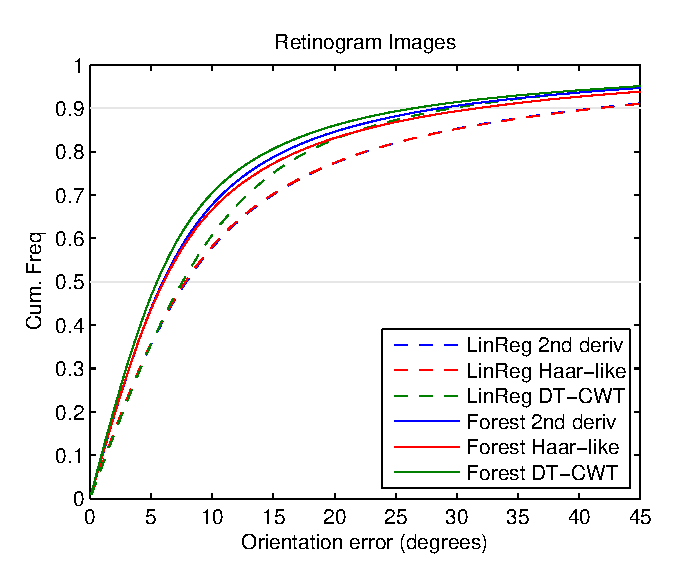
\includegraphics[width=0.48\columnwidth]{\figpath/retina/retinogram_expt}
%
\caption{Cumulative frequency of angular error for retinogram images.}
\label{f:cumfreq}
\end{figure} % from BMVC
\begin{figure}[t]
\centering
\def\figwidth{0.48\columnwidth}
\begin{tabular}{@{}c c@{}}
\includegraphics[width=\figwidth]{\figpath/retina/cumfreq} &
\includegraphics[width=\figwidth]{\figpath/retina/thickness_vs_error-summ} \\
(a) & (b)\\
\includegraphics[width=\figwidth]{\figpath/retina/contrast_vs_error-summ} &
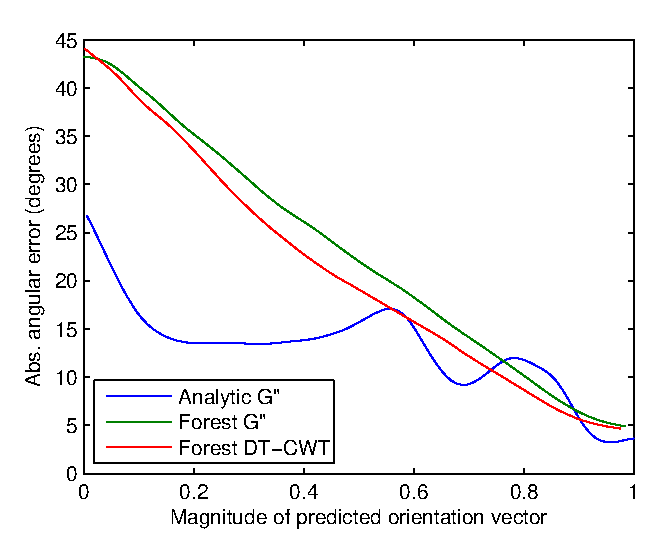
\includegraphics[width=\figwidth]{\figpath/retina/response_vs_error_ret} \\
(c) & (d)\\
\noalign{\smallskip}
\end{tabular}
%
\caption{Orientation estimation results for selected methods over pixels along the centre of the vessel: (a) Cumulative frequency of angular error; (b) Kernel estimate of mean error with respect to line thickness; (c) Kernel estimate of mean error with respect to line contrast; (d) Kernel estimate of mean error with respect to predicted orientation magnitude (for the analytic Gaussian, the absolute response scaled between 0 and 1 at the maximal angles is used).}
\label{f:retina_graphs}
\end{figure}

\comment{Some measure of spread for these figures, or a box plot to show significance.}
 % from MICCAI

% Discussions

\subsubsection{Choice of feature}
\label{s:exp_retinogram_orientation_wrt_feature}
% Compare all feature types with the most powerful and flexible regressor (e.g. Random Forests) so that complex feature types are not disadvantaged.

Features based on odd filters -- first derivatives of the Gaussian and the monogenic signal, for example -- were consistently outperformed by those that included even filters (\fref{f:retina_graphs}). This can be attributed to the high errors that occur when using only odd filters at the centre of a vessel where there is little or no image gradient; this failure is particularly acute for the most narrow vessels, consisting of a single pixel, where the whole vessel is a centreline by definition. 

Of the two features that use even filtering -- the second Gaussian derivatives and the \dtcwt{} -- the \dtcwt{} provided better estimates under most conditions. This suggests that using both odd and even filters (such that phase information becomes available) does indeed improve performance, though at a cost in computational demand.

%With the exception of the boosted regressor, the Haar-like approximation exhibited similar performance to the second derivative, suggesting that it may be used effectively in scenarios where efficiency is a concern.




\subsubsection{Choice of regressor}
\label{s:exp_retinogram_orientation_wrt_regressor}
% Compare all regressors with a given input feature (preferably the richest - dtcwt)
%
Comparing the performance of all estimation methods for a fixed input feature type (the \dtcwt{}), orientation was consistently estimated more accurately by regression compared to the analytic method with particular improvement seen in faint narrow vessels. 

Moreover, complex regressors such as Random Forests outperformed simpler ones such as linear regression. This suggests that the relationship between responses to the \dtcwt{} and line orientation is nonlinear.

Our use of statistical learning approaches was motivated threefold: by their ability to pool over scales and local neighbourhoods; to combine filter responses where an analytic solution was not obvious (when using the \dtcwt{}, for example); and to model data-dependent properties such as image noise and the observed distribution of line widths and contrasts. 

% Linear regression
%As noted earlier, when using second derivative responses it is necessary to compute the responses at the two possible solutions to determine which is the correct one. Since the linear regressor minimizes the average error, however, it contains no mechanism for selecting the correct orientation and this is likely to be one reason for its poor performance relative to more sophisticated regressors such as the Random Forest.


\subsubsection{Effect of window size}
\label{s:exp_retinogram_orientation_wrt_window_size}
Pooling results over a local neighbourhood by stacking filter responses into a single vector also had a significant effect on error rates. This was particularly the case for features based on odd filter responses, since it reduces the effect of small gradients at the centre-line by pooling estimates from nearby pixels with stronger gradients and therefore better estimates.

We also note that second Gaussian derivatives can be closely approximated using finite differencing of a first Gaussian derivative. Therefore, a linear regression over first derivative responses at neighbouring pixels is able to replicate the errors of the method based on second derivatives.


\subsubsection{Effects of line thickness}
\label{s:exp_retinogram_orientation_wrt_width}
% Compute orientation errors for lines of different widths
%
Because narrow vessels are interesting but occupy a small proportion of the vessel map, here we provide a breakdown of orientation errors for lines of different widths. To estimate the vessel widths, we computed the distance transform of the known vessel mask and set the width at every vessel pixels to that of the nearest centreline pixel.

\begin{figure}[t]
\centering
\def\figwidth{0.75\columnwidth}
\includegraphics[width=\figwidth]{\figpath/retina/thickness_vs_error-summ} 
%
\caption{Orientation estimation results for selected methods over pixels along the centre of the vessel: Kernel estimate of mean error with respect to line thickness.}
\label{f:retinogram_orientation_wrt_width}
\end{figure}

We visualize this relationship using a one dimensional kernel smoother (\fref{f:retinogram_orientation_wrt_width}) and see that errors are similar for the thicker vessels (where there is more image information with which to estimate orientation and thus we expect all methods to perform well) but that the regression reduces error considerably for the narrower vessels. Interpreting results for vessels with a width of more than approximately 12 pixels is difficult because they are rare, which leads to high variability in the kernel estimate of error, and because the vessel width exceeds the central region of our largest filter. These vessels, however, are typically of less interest to the retinopathy community.


\subsubsection{Effects of line contrast}
To do so, we defined line contrast as the absolute difference between the vessel intensity and the mean intensity of background pixels in a $15{\times}15$ neighbourhood.

We see a similar effect when considering the distribution of error with respect to line contrast (\fref{f:retina_graphs}c): the learnt regressors outperform analytic methods especially on lines with low contrast though there is little significant difference between the methods for vessels of greater contrast. We also see errors begin to increase beyond a certain contrast, though this is most likely due again to the rarity of high contrast vessels and the correlation of high contrast with large width.

% We conclude that...?
Overall, combining \dtcwt{} features with Random Forest regression was most successful with the \dtcwt{} in particular benefiting from the improvement of Random Forests over simple linear regression (\tref{t:retinopathy})



\clearpage
\section{Application: Mammography}
[Notes on prevalance and incidence of breast cancer, its effect on mortality, and the economic costs of treatment at later stages.]

\subsection{Datasets}
\subsubsection{Real Mammograms}
\label{dataset_realmamm}
%
Our database of real mammograms consisted of a sequential set of 84 abnormal mammograms with biopsy-proven malignancy, drawn from a screening population (Nightingale Breast Centre, South Manchester University Hospitals Trust, UK), and 89 normal mammograms from the same individuals, but of the contralateral breast (where disease was radiologically confirmed to be confined to one breast). All mammograms were digitised to a resolution of $90 \mu\text{m}$ using a Vidar CADPRO scanner. A $4 \by 4$ cm ($512 \by 512$ pixel) patch was then extracted around each abnormality, and a similar patch sampled randomly from each of the normal mammograms (\fref{f:real_examples}).

For each abnormal patch, an expert radiologist manually annotated 555 (not necessarily all) of the spicules associated with the abnormality, using in-house software. Though these expert spicule annotations were not sufficiently accurate to be used directly, we used them as a basis for selecting spicule pixels by initialising a snake~\cite{Kass_etal_IJCV88} with each original annotation, and iterating it to convergence using evidence from the \comment{linear structure probability?} image~\cite{Muralidhar_etal_TMI10}. In total, the 555 refined spicules identified 36\,514 spicule pixels.

\subsubsection{Synthetic Mammogram-like Images}
\label{s:dataset_synthmamm}
%
Given the practical difficulties of obtaining a precise binary labelling of curvilinear structure in real mammograms, we generated synthetic images~\cite{Berks_PhD10} with which to train and test algorithms for analysis. Specifically, to create each image we took a $4 \by 4$ cm ($512 \by 512$ pixel) region from a randomly selected real mammogram with 256 grey levels, and filtered out the high frequency linear structures, leaving only the coarse background texture with local image noise across all frequencies. We then superimposed linear structures with randomly chosen parameters (orientation, width, peak intensity and profile shape) onto the background.

\begin{itemize}
\item Orientations were drawn from a uniform distribution over the range [0, $\pi$] radians.

\item Widths were drawn from a uniform distribution over [4, 16] pixels.

\item Peak intensity [1,255] grey-levels (relative to images scaled 0-255) from an exponential distribution with half-width 4 grey-levels;

\item Profile shape $S$ determined by the equation $S = a + (1-a) \sin(x)$ for offsets $x \in (0,\pi)$, where the 'squareness' parameter $a$ determines how close the shape is to a pure half-cycle $\sin$ or a rectangle and is drawn uniformly from [0,1].
\end{itemize}

The result was an image whose statistics were close to those of a real mammogram, but with known line parameters (\fref{f:synthetic_responses}).

In this manner, we generated 10\,460 training images and 4\,903 test image patches using 72 training and 30 test normal\comment{normal?} mammograms.

The literature suggests (and we ourselves observed) that the best performance is obtained by training with a balanced dataset -- in this case with the same number of foreground (curvilinear structure) and background examples. Having created these images, therefore, we sampled feature vectors at pixels on the centrelines of the superimposed linear structure, and an equal number of `background' pixels to serve as positive and negative training sets, respectively.\comment{for detection, of course} 

During training, backgrounds were randomly sampled from the 10\,460 training patches and a single line was added to the centre of the patch. These images were produced 'on-the-fly' during each tree-building step of random forest construction and no permanent set was maintained. 

(We simply generated images until we had the desired 200k points, then built the tree; we did this for 200 trees.)

For testing, 100 backgrounds were randomly selected from the test patches. To each, multiple lines were added sequentially, with the number and position of lines varying randomly.



\subsection{System Parameters}
During training, we synthesized random line images to construct a new training sample at each tree-building step rather than using a single set of training data from which samples were drawn with replacement (\ie bootstrapping). For detection, each sample comprised 100\,000 curvilinear structure pixels and 100\,000 background pixels, while for orientation regression we used 200\,000 pixels all belonging to curvilinear structure. 

Random Forest building proceeded exactly as in the retinography experiments.

For the four learning methods (\dtcwt{}/RF, Monogenic/RF, Linop/RF, Gaussian/RF), we first constructed random forests to classify between structure and background pixels.

For any given representation (\dtcwt{}, Monogenic, Linop, Gaussian) and forest (classification, regression) we applied the following scheme:

\begin{enumerate}
\item	Generate a new synthetic line image with known ground truth
\item Extract feature vectors for a random set of pixels in the image
\item Repeat 1 and 2 until training sample complete
\item Construct tree using the CART algorithm
\item Repeat 1 to 4 until 200 trees constructed
\end{enumerate}

For all methods, the number of scales used $s$ and the neighbourhood size $w$ were empirically tested to select the best combination for each method. In each case, we tried $s$ = 3, 4, 5, 6 and $w$ = 1, 3.

\begin{itemize}
\item	\dtcwt{}/RF: images were decomposed using the \dtcwt{} to $s$ scales. Neighbourhoods of interpolated phase and magnitude coefficients were extracted in each of the 6 oriented subbands producing a feature vector of $12 \cdot w^2 \cdot s$ elements.

\item	Monogenic/RF: the monogenic signal was extracted across $s$ scales, with the initial wavelength set at $\lambda$ = 4 pixels. Neighbourhoods of phase, amplitude and orientation values were computed giving a total feature size of $6 \cdot w^2 \cdot s$. 

\item	Linop/RF: 8 oriented line filters were computed at each scale. Collecting neighbourhoods of the oriented filter responses produced $16 \cdot w^2 \cdot s$ elements in each feature vectors.

\item	Gaussian/RF: for the Gaussian 2nd derivative method, the three directional derivatives were applied to an image at each scale. The standard deviation of the smallest kernel was 1 pixel, subsequent kernels increased by a factor of 2 at each scale. As with Monogenic/RF this resulted in feature vectors with $6 \cdot w \cdot s$ elements.
\end{itemize}

For testing, feature vectors for each representation were extracted at all pixels in the 100 synthetic test images.


\subsection{Detecting Linear Structures}
In our first set of experiments, we investigate the ability of each image representation and classification method to detect the presence of a line (such as a vessel, duct or spicule) in the image. For this task, we used a binary label (present \vs{} not present) as the target we aimed to predict.

\subsubsection{Results on Synthetic Mammograms}
%begin IPMI
To show qualitative results for real mammograms, the seven methods were applied to detect curvilinear structures in the malignant regions. Example detection results are shown in \ref{f:}.

\comment{The following is very waffly.}
\comment{In terms of applying the learning methods to real images, it is worth noting how the methods scale with increasing image size -- particularly above the point at which the set of feature vectors for all image pixels can be stored in working memory. For the \dtcwt{}, provided the initial decomposition can be stored in memory (which, due to its low-redundant decimating construction, is possible even for full size mammograms of the order $3000 \by 2400$ pixels) then interpolated coefficients can be efficiently sampled to generate feature vectors for block-wise regions of the image. Each block of feature vectors can be classified by the forest and cleared from working from memory storing only the output of the forest. In this way only a small overhead is introduced for block-wise classifying the image. 

However, for the other methods it becomes necessary to interleave the decomposition of the image with the sampling of feature vectors. For example, it may be necessary to apply the filters at a single scale, extract features for that scale for a particular block of the image, filter at the next scale and extract those features, and so on. Of course, when the complete feature vectors for a single block have been classified, the process repeats. Thus a large image may in fact end up by decomposed many times over introducing a large computational overhead for block-wise processing. The point at which this cost occurs will depend on the size of the image and the type of representation used. The cost is worst for Linop which requires storing 8 (\ie~the number orientations) full copies of the image at each scale, compared to just 3 for the Gaussian and Monogenic methods.}
%end IPMI
 % IPMI, IWDM

\subsubsection{Results on Real Mammograms}
The classification and regression forests were then used to compute a line detection score (the proportion of votes for the curvilinear structure class) at each pixel. 

In addition to the four learning methods, the prescriptive variants of the Monogenic, Linop and Gaussian approaches were applied to the test images (\ref{f:synthetic_responses}).

ROC curves for the seven methods tested are shown in~\ref{f:}, using the known ground-truth for the test images to define pixels on the centrelines of curvilinear structures as foreground, and pixels lying outside the structures as background. Areas under the ROC curves and detection sensitivities at a fixed specificity of 90\% are shown in~\ref{t:}.

As expected, because Linop, of the three prescriptive methods, discards the highest proportion of filter responses, Linop/RF gains the most from training. This highlights the ability of the random forests to extract useful information from a rich local description of image content, and whilst we do not have a prescriptive variant to compare it to, we believe this shows the importance of training in maximizing the benefit of using the \dtcwt{}. 

We also note that the added information that can be gained from the \dtcwt{} representation results from an increase in the richness of the local description of texture and is not due to increasing the support of the descriptor. Indeed, as described above we tested all representations over an equivalent range of filter scales so that the same image support was available to each method.

%\begin{table}
\centering
\caption{Line detection and orientation computation results. For every algorithm, we present the area under the ROC curve ($A_z$), the sensitivity at 90\% specificity, and the mean absolute error of the orientation estimate.}
\label{t:line_detection}
%
\begin{tabular}{l c c c}
Algorithm	
		& $A_z$							& Sens. \@ 90\% spec. & MAE \\
\hline
\dtcwt{}/RF ($w$ = 1, $s$ = 5)												
		& 0.923$\pm$0.00036	& 0.792 							& 15.88 \\
Linop/RF ($w$ = 1, $s$ = 5, 8 orientations)				
		& 0.911$\pm$0.00048	& 0.757								& 19.35 \\
Gaussian/RF ($w$ = 1, $s$ = 4, $\sigma_{min}$ = 1)
		& 0.901$\pm$0.00048	& 0.731								& 21.37 \\
Monogenic/RF ($w$ = 1, $s$ = 4, $\lambda$ = 4)
		& 0.868$\pm$0.00045	& 0.643								& 33.73 \\
Monogenic ($s$ = 3, $\lambda$ = 4)									
		& 0.818$\pm$0.00055	& 0.547								& 30.86 \\
Gaussian ($s$ = 4, $\sigma_{min}$ = 1)							
		& 0.813$\pm$0.00053	& 0.533								& 24.27 \\
Linop ($s$ = 5, 8 orientations)										
		& 0.737$\pm$0.00060	& 0.413								& 29.32 \\
\end{tabular}
\end{table}
 % IWDM, IPMI

\subsection{Classifying Spicules}
\label{s:exp_realmamm_spicule_classification}
%
Although it was not realistic to create a training set of mammogram images with all spicules annotated, we were able to obtain expert annotations of a reasonably large number of spicules in a set of mammogram patches containing malignant tumours. These annotations were used to select pixels for the positive training set. 

To create a balanced training set we sampled feature vectors from the same number of pixels in a set of normal mammogram patches, such that the distribution of curvilinear structure probabilities was the same as for the spicule training set.

Having trained a classifier using the synthetic data, we can classify feature vectors extracted about every pixel in a synthetic or real mammogram image to obtain a line probability image (using the probabilistic labelling scheme as opposed to a hard binary classification).

The four learning-based methods were also applied to the problem of spicule/non-spicule classification. Feature vectors were formed as above, and random forest classifiers were trained using balanced spicule/non-spicule training data. 

% Cross validation
To make effective use of the available data, we used a 10-fold cross validation design. The set of normal and abnormal regions were divided into 10 groups so that the total number of normal and spicule pixels in each group were as close as possible to one tenth of the total and no two views from the same case were included in different groups. The samples in each group were then classified using a random forest trained on the samples from the remaining 9 groups. The classification results from each group were pooled to generate an unbiased class probability for each sampled pixel. 

These probabilities were used to compute an ROC curve for each training regime, and the area under the curve ($A_z$) was computed and used as a measure of classification performance. The ROC curves and $A_z$ values for the three methods are shown in \ref{f:} and \ref{t:}. These results demonstrate a clear advantage for \dtcwt{}/RF. Linop and Gaussian representations perform significantly worse than the two representations that do include phase; we believe that this is because phase information captures profile shape.

In addition to computing a class vote for spicule membership at only those pixels in the selected training sets, the forests we have constructed can be used to compute results for whole region in each cross-fold group. Typical qualitative \dtcwt{}/RF results for a normal and abnormal region are shown in \ref{f:}. In the left column, the original regions are shown. The spiculations of the mass are clear and well defined, particularly to the lower right of the central mass. In the normal region, a set of structures intersect in an approximate radial pattern that may trigger a feature detector erroneously. In the right column, the predicted spicule class membership is shown as hue varying from cyan (normal) to pink (spicule), modulated by the \textbf{output of the \dtcwt{}/RF detection method}. Note how the linear structures in the region of the mass are deemed highly likely to be spicules, while those in the normal region are not. 
%This shows excellent promise as a means of providing a relevance measure to methods for abnormality detection.

% IMPI Figure 5

\begin{figure}
\centering
\begin{tabular}{c c}
\includegraphics[width=\qtrcol]{\figpath/mammo/ipmi/mass046} &
\includegraphics[width=\qtrcol]{\figpath/mammo/ipmi/norm068} \\
(a) & (b) \\
\includegraphics[width=\qtrcol]{\figpath/mammo/ipmi/spic_prob_mass046_a} &
\includegraphics[width=\qtrcol]{\figpath/mammo/ipmi/spic_prob_norm068_a} \\
(c) & (d)
\end{tabular}
%
\caption{Regions depicting (a) malignant and (b) normal tissue. The corresponding spicule classification results are depicted in (c,d) using hue to indicate abnormality -- ranging from cyan (normal) to pink (spicule) -- and intensity to indicate the line detection output from the DT-CWT method.}
\label{f:mammogram_examples}
\end{figure}



\subsection{Estimating Orientations}
As the lines were synthetic, we had access to both a mask (\fref{f:synth_mammography}b) and ground truth orientation for the superimposed structure.

Unlike other similar studies~\cite{Berks_etal_IPMI11}, we do not require a negative classification of background pixels and therefore do not need to remove existing real structures from the images. As a result, the synthetic lines will be disrupted by any existing image structure and thus the dataset presents a much tougher and more realistic test of orientation estimation than shown in, for example,~\cite{Berks_etal_IPMI11}.

We sampled 200\,000 pixels from such images and computed a feature vector for each with which we trained a regressor. We then applied every trained regressor for every feature type to a fixed set of 100 synthesized images (generated from mammographic backgrounds not used in training) and computed the error at the known line pixel positions. As before, Random Forests and the \dtcwt{} outperform other methods, though errors were generally higher on account of the more challenging data (\fref{f:mammo_graphs}a and \tref{t:synth_mammography}). We also note that although the median error for the Random Forest was lower for the \dtcwt~than the second derivatives, the situation was reversed for higher percentiles (\ie~the graphs cross). We care less, however, about differences between errors above a certain threshold (it matters little whether the estimate is out by $60^\circ$ or $70^\circ$ -- they are both terrible estimates) so it may be argued that the Random Forest performs better over the region in which we are interested.

For orientation, only pixels belonging to curvilinear structures (although not necessarily at the centerline) were included in the results. The absolute differences between the predicted and known orientations (with appropriate angle wrapping) were taken, and used to generate cumulative distribution functions of orientation errors for each method, as shown in~\ref{f:}. The mean absolute errors of the estimated orientations are also included in~\ref{t:}.

%\input{figs/fig_synth_mammograms.tex}
%% CVPR Figure 5

\begin{figure}[t]
\centering
\begin{tabular}{@{}c c@{}}
\includegraphics[width=0.47\columnwidth]{\figpath/mammo/024RCC_roi_crop} &
\includegraphics[width=0.47\columnwidth]{\figpath/mammo/024RCC_roi_class_ori_crop} \\
(a) & (b) \\
\noalign{\smallskip}
\end{tabular}
%
\caption{Real mammographic images: %
(a) input image; %
(b) estimated orientation from a Random Forest using \dtcwt{} features. Hue indicates the estimated orientation and brightness is determined by the confidence in the estimate (as quantified by the magnitude of the predicted orientation vector).}
\label{f:real_mammography}
\end{figure}

%\begin{table}[t]
\centering
\begin{tabular}{l c c c c}
\toprule
							& \multicolumn{4}{c}{Feature Type} \\
							& $G'$		& $G''$	& Mono.				& \dtcwt \\
\cmidrule{2-5}
\input{mammography_table.txt}
\bottomrule
\noalign{\smallskip}
\end{tabular}
%
\caption{Median absolute error (degrees) for combinations of input feature and {3{$\times$}3} regressor on 100 synthetic mammogram images.}
\label{t:synth_mammography}
\end{table}

%CVPR Figure 4

\begin{figure}[t]
\centering
\begin{tabular}{c c}
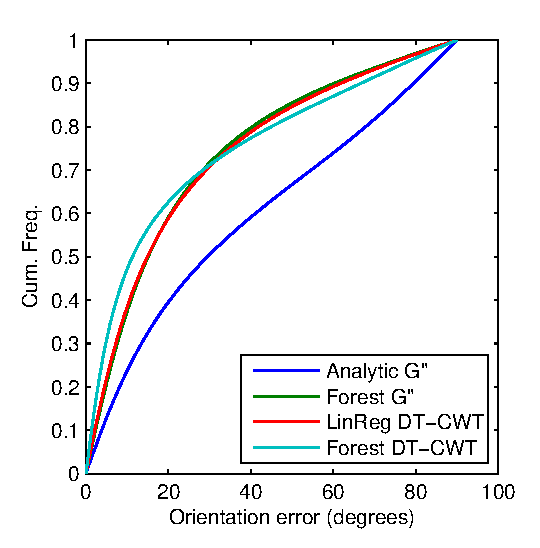
\includegraphics[width=0.47\columnwidth]{\figpath/mammo/cdf_error_mammo} &
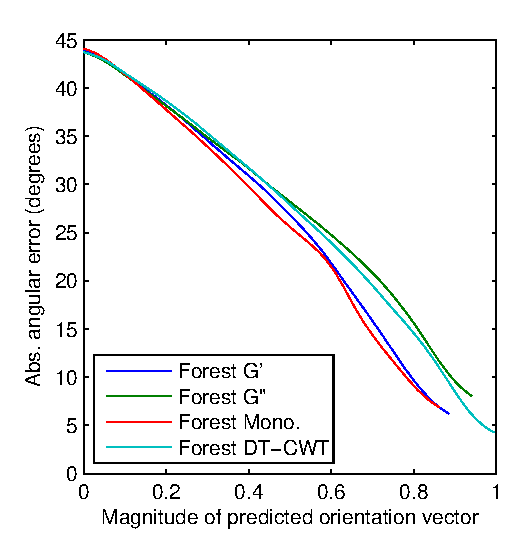
\includegraphics[width=0.46\columnwidth]{\figpath/mammo/response_vs_error_mammo} \\
(a) & (b) \\
\noalign{\smallskip}
\end{tabular}
%
\caption{Mammogram results for four selected methods: (a) Cumulative frequency of angular error; (b) Kernel estimate of mean error with respect to the magnitude of the orientation vector predicted by the forest.}
\label{f:mammo_graphs}
\end{figure}


In \fref{f:mammo_graphs}b we show the kernel estimate of mean angular error with respect to the magnitude of the orientation vector predicted by the forest trained on each feature type. Recall that this magnitude encodes the mean angular dispersion of the training data arriving the leaf nodes used in making each orientation prediction. That this magnitude acts as a measure of confidence in its prediction is evidenced by consistent reduction in angular error with increasing magnitude for all feature types. The magnitudes can be used to weight each orientation prediction in further processing and may be preferable to a similar feature such as the absolute response returned from the analytic combination of the Gaussian derivatives. This is because the latter is essentially a measure of image contrast at a structure of interest. So for example, if there are two lines, one of which has double the contrast of the other, the magnitude of the filter response will also double, even if the orientation may measured equally accurately in both lines. Similarly, a very bright or very dark spot in the image will also produce a strong filter response where in fact orientation can't be reliably estimated.

% CLAIM: that the separable filters are faster than nonseparable ones (but by how much?)
% CLAIM: that the Haar-like features are faster than separable filtering
In terms of efficiency, we recorded the mean time (using Matlab on a 2.66Ghz, quad-core desktop PC with 3.25Gb RAM) over 20 images for five feature representations: 
the monogenic signal (2.96\emph{s}); 
%non-separable second derivatives (3.71\emph{s}); 
separable second derivatives (2.04\emph{s}); 
%their Haar-like approximations (2.35\emph{s}); 
and the \dtcwt{} (19.96\emph{s}). 
%
Unsurprisingly, under test conditions 
%the separable filters were indeed faster than their non-separable counterparts while 
the \dtcwt{} was an order of magnitude slower than the separable filters. 
%
%The Haar-like approximations were comparable to but slower than the separable filters, though the separable filters did exploit the built-in (\ie~compiled) convolution functions in Matlab; we expect that an optimized implementation of the Haar-like features would offer similar performance gains as observed in face detection applications~\cite{Viola_Jones_IJCV04}.
%
%%% This is a pretty weak conclusion to the experiment but the best we can expect at this point. Also, if you need to use a regressor as slow as the RF to get accuracy that is comparable to the analytic second derivatives then the small difference in filtering time becomes irrelevant}

%begin IPMI
The orientation results for both Monogenic and Monogenic/RF were surprisingly poor. Counter-intuitively, visual analysis of the test outputs showed that the Monogenic methods performed particularly badly at the exact centerline of curvilinear structures, where an essentially random orientation appeared to be returned. This is in contrast to the other tested methods that, as expected, performed strongest along the centerlines of structures. Computing estimation errors at pixels belonging to structures but not lying on the centerline produces a small improvement in the results (mean absolute errors of $32.55 \deg$ and $29.39 \deg$ for the RF and prescriptive variant respectively), though even then performance lags behind the other tested methods and of course in a real image we do not know the precise location of structure centerlines. 
%end IPMI

These results show that the four learning methods perform significantly better than the three prescriptive methods (with the exception of orientation computation in Monogenic/RF). \dtcwt{}/RF is significantly the strongest performing for both line detection and orientation estimation, followed by Linop/RF then Gaussian/RF.

%\input{figs/fig_cumfreq_orientation_error.tex}
%\begin{table}[t]
\centering
\begin{tabular}{l|c c c c}
							& \multicolumn{4}{c}{Feature Type} \\
							& Monogenic		& 2nd deriv.	& Haar				& \dtcwt{} \\
\hline
\input{mammography_table.txt}
\end{tabular}
%
\caption{Median absolute error (degrees) for combinations of input feature and regressor on 100 synthetic mammogram images.}
\label{t:synth_mammography}
\end{table}


%\begin{table}
\centering
\caption{Line detection and orientation computation results. For every algorithm, we present the area under the ROC curve ($A_z$), the sensitivity at 90\% specificity, and the mean absolute error of the orientation estimate.}
\label{t:line_detection}
%
\begin{tabular}{l c c c}
Algorithm	
		& $A_z$							& Sens. \@ 90\% spec. & MAE \\
\hline
\dtcwt{}/RF ($w$ = 1, $s$ = 5)												
		& 0.923$\pm$0.00036	& 0.792 							& 15.88 \\
Linop/RF ($w$ = 1, $s$ = 5, 8 orientations)				
		& 0.911$\pm$0.00048	& 0.757								& 19.35 \\
Gaussian/RF ($w$ = 1, $s$ = 4, $\sigma_{min}$ = 1)
		& 0.901$\pm$0.00048	& 0.731								& 21.37 \\
Monogenic/RF ($w$ = 1, $s$ = 4, $\lambda$ = 4)
		& 0.868$\pm$0.00045	& 0.643								& 33.73 \\
Monogenic ($s$ = 3, $\lambda$ = 4)									
		& 0.818$\pm$0.00055	& 0.547								& 30.86 \\
Gaussian ($s$ = 4, $\sigma_{min}$ = 1)							
		& 0.813$\pm$0.00053	& 0.533								& 24.27 \\
Linop ($s$ = 5, 8 orientations)										
		& 0.737$\pm$0.00060	& 0.413								& 29.32 \\
\end{tabular}
\end{table}
%\input{figs/fig_synth_mammograms.tex}
%% CVPR Figure 5

\begin{figure}[t]
\centering
\begin{tabular}{@{}c c@{}}
\includegraphics[width=0.47\columnwidth]{\figpath/mammo/024RCC_roi_crop} &
\includegraphics[width=0.47\columnwidth]{\figpath/mammo/024RCC_roi_class_ori_crop} \\
(a) & (b) \\
\noalign{\smallskip}
\end{tabular}
%
\caption{Real mammographic images: %
(a) input image; %
(b) estimated orientation from a Random Forest using \dtcwt{} features. Hue indicates the estimated orientation and brightness is determined by the confidence in the estimate (as quantified by the magnitude of the predicted orientation vector).}
\label{f:real_mammography}
\end{figure}



\clearpage
\section{Discussion}
\label{s:discussion}

\begin{itemize}
\item Combining first and second derivatives: firsts are good at edges, seconds are good at line centres - they complement each other.

\item Discussion about linear regression coefficients: how they take a sinusoidal appearance, how we need to choose between two discrete orientations (which is not possible with a `vanilla' linear regressor)
%
\begin{figure}[t]
	\centering
		\includegraphics[width=0.9\columnwidth]{\figpath/linreg_coeffs}
	\caption{Linear regression coefficients for (left) $\cos 2\theta$ and (right) $\sin 2\theta$, using (top) response magnitude and (bottom) response phase.}
	\label{f:linreg_coeffs}
\end{figure}
%
\item Logistic regression can be used to limit the output to -1..+1. Boosted regression implicitly does the same by predicting only what it has seen before. These limits, however, are applied to sinT and cosT independently which means you can still get values outside of the unit circle.

\item Random Forest classifier/regressor has lots of details to get right, not least in making sure that the orientations wrap around correctly. Also differences in how the branches are split etc.
\end{itemize}

The results of our experimental evaluation are extremely encouraging, and represent a significant improvement over the current state of the art.

Although learning accounts for a significant part of this improvement, the choice of representation is also important and will have a different effect on performance depending on the task in hand. For example, constructing a representation based on the raw responses to Linop filters produces features that are excellent for estimating structure orientation but provide less information for determining structure shape and thus type.

Conversely, features formed from the monogenic signal are good at determining structure type - most likely because of the inclusion of the phase measure - while they perform relatively poorly at detection and orientation estimation.

For these reasons, it seems fair to conclude that the \dtcwt{} provides the best all round representation. It produced the strongest performance for all three tasks (curvilinear structure detection, orientation estimation and spicule classification). Moreover, the \dtcwt{} incurs the least overhead when working with full-size real images that require block-wise classification/regression. For example, initial tests show that the structure detection and orientation regression can be performed on a full-size (approximately $3000 \times 2400$ pixels) mammogram in approximately 1hr 30mins.

We show that, overall, our approach is significantly better than the current state-of-the-art, and that we can distinguish effectively between curvilinear structures associated with malignancy (spicules) and those associated with normal structure (vessels, ducts etc).




We have presented a discriminative learning-based approach to the detection and classification of curvilinear structures, based on a combination of \dtcwt{} representation of local structure and random forest classification. We have applied the method to the challenging problem of detecting and estimating the orientation of curvilinear structures in mammograms and distinguishing between normal and abnormal structures. The results of our experimental evaluation are extremely encouraging, and represent a significant improvement over the current state of the art.

We have also introduced learning-based variants of three existing methods, demonstrating that whilst learning accounts for a significant part of this improvement, the choice of representation is also important and will have a different effect on performance depending on the task in hand. For example, constructing a representation based on the raw responses to Linop filters produces features that are excellent for estimating structure orientation but provide less information for determining structure shape and thus type. Conversely, features formed from the monogenic signal are good at determining structure type - most likely because of the inclusion of the phase measure - whilst they perform relatively poorly at detection and orientation estimation. For these reasons, it seems fair to conclude that the \dtcwt{} provides the best all round representation. It produced the strongest performance for all three tasks (curvilinear structure detection, orientation estimation and spicule classification). Moreover, as discussed in section 5.2, of all the methods, the DT-CWT incurs the least overhead when working with full-size real images that require block-wise classification/regression. For example, initial tests show that the structure detection and orientation regression can be performed on a full-size (~3000 x 2400 pixels) mammogram in ~1hr 30mins.

Our next goal is to show that improving the individual steps of curvilinear structure and orientation estimation result in a subsequent improvement for a high level task such as detecting patterns of spiculations indicative of disease. Moreover we hope to show that classification into structure type can further aid such tasks by focusing only (or at least more) on those structures most likely to be associated with disease. 


\clearpage
\section{Conclusions}
In conclusion, we see that filters based only on odd filters perform poorly near the centre of a curvilinear structures whereas even filters such as the second derivatives are much better, though a feature set comprising the responses to both odd and even filters offers further advantages. 
There is also potential to approximate the second derivative filter responses with Haar-like features if efficiency is a key concern, though it is less clear how to combine these responses to give a unique solution. 
Of the filters we tested, we found that the \dtcwt{} gave the best results regardless of the regressor used, though was significantly more computationally expensive. Of the regressors we tested, Random Forests performed best and we have provided some insight as to why alternatives (\eg~linear regression) perform less well. 
Combining suitable filters with Random Forests produces vessel segmentation that matches the state of the art without application specific post-processing as used in rival methods (and that we would expect to improve results further). 
Moreover, we have shown that regressing orientation estimates using similar machinery is more accurate than relying on analytical estimations. 
Though demonstrated on retinograms, our methods are generally applicable to linear structures in any images where ground truth is available.
Most promisingly, we note the larger improvement in orientation estimation for particularly challenging structures such as thin, low-contrast vessels. As a further advantage of regressing with random forests, we propose that both the predicted orientation \emph{and} its associated magnitude may be useful features in further processing.
\comment{We must, however, take care when building regressors for orientation prediction in order to ensure that angles wrap around the circle correctly.}


\section*{Acknowledgements}
We thank Nick Kingsbury for the \dtcwt{} Matlab toolbox. Mammograms were provided by the Nightingale Breast Centre, South Manchester University Hospitals Trust, UK and were annotated by Dr Caroline Boggis and Dr Rumana Rahim. This work was funded by EPSRC grant EP/E031307/1.

\bibliographystyle{plain}
\bibliography{%
./bib/_aliases,%
./bib/mobio,%
./bib/mammography,%
./bib/ml,%
./bib/nailfold,%
./bib/papers_by_year,%
./bib/local}

\end{document}